\textbf{Introduction}
The purpose of this test was to see if the GPS spoofing worked when the drone was airborn. The same hardware and software were used as in section \ref{sec:test_of_spoofed_positions_indoore}, though with a few changes.

The GPS used in test 1 to collect coordinates were mounted on the EduQuad.

The idea was to pass-through the GPS coordinates from the Neo 6-P GPS to AQ. If the CAN spoofing works as expected the drone should behave normally when flying in position-hold mode.

\textbf{Test}

Figure \ref{fig:eduquad_bottom_up} shows how the hardware were mounted on the EduQuad. It was temporary mounted with strips and tape to avoid short circuiting. \Mathias{Opdater billede med test-equipment} 

In test 1 the altitude of the drone was hardcoded since it had no relevance  in the test. Though in test 2 if was necessary since the UKF\footnote{\url{https://github.com/bn999/autoquad/blob/master/onboard/run.c\#L111}} uses the altitude from the GPS to estimate the position of the drone. Furthermore the following check where inserted to make sure only valid GPS coordinates were fed into the AQ:
\begin{center}

\begin{minipage}{\textwidth}
		\begin{lstlisting}[language = c++, caption = Quality checks added to discard bad positions, label=code:pseudo_tx]
// default low accuracy
gpsData.hAcc = 5; // Meters
gpsData.vAcc = 5; // Meters

if(gpsData.fix == 1){ // Single point solution
	if(gpsData.hdop < 3){
		if(gpsData.satellites >= 5){
			AQ_PRINTF("Recv. Valid GPGGA\n",0);
			// High accuracy
			gpsData.hAcc = 2.5; // Meters
			gpsData.vAcc = 2.5; // Meters
			// Set flag to process new message
			CoSetFlag(gpsData.gpsPosFromCanFlag);
        } else {
			AQ_PRINTF("Satellites: %f \n", gpsData.satellites);       
        }
    } else {
	    AQ_PRINTF("HDOP: %f\n", gpsData.hdop);    	
    }
} else {
	AQ_PRINTF("Fix: %f\n", gpsData.fix);
}
		\end{lstlisting}
\end{minipage}
\end{center}

\begin{figure}[H]
    \center
    \includegraphics[width=0.6\textwidth]{graphics/test_outdoore_mounts.eps}
  \caption{The EduQuad drone with the hardware used in the test}
    \label{fig:eduquad_bottom_up}
\end{figure}
An extra battery was mounted on the drone to supply the Rpi. The ROS nodes running on the Rpi had to be start up before AQ starts registering notes on the CAN-bus. If the nodes was not started up, they would not reply to AQs reset-msg it sends when it is booting. \\

When the ROS-node were connected to the CAN bus, it showed that the ROS-node needed extra checking on CAN messages in order to detect difference between messages targeted the ROS-node and messages targeted the ESC32-nodes.


A bug in the \textit{can\_socketcan} -node used to communicate with the Peak-Can adapter where found a fixed. It was later on merged back into Frobomind \footnote{\url{https://github.com/FroboLab/frobomind/pull/12}}
\textbf{Conclusion} \\

The test did not go as expected. The test was carried out under a time pressure since the author's supervisor only had 30 minutes to carry out the test.

The author did though gain experience when having multiple CAN devices connected to the CAN-bus.

Several things went wrong through the test:
\begin{itemize}
	\item The onboard GPS was not disabled
	\item The author accidentally forgot to set the DOP values used in AQ
	\item No reference flight after the firmware were flashed for the first time.
	\item The GPS antenna was not mounted in the middle of the frame as the onboard antenna.
\end{itemize}

Figure \ref{fig:qground_station_dop} shows the DOP value is lowering witch indicates that AQ was using its onboard GPS.

\begin{figure}[H]
    \center
    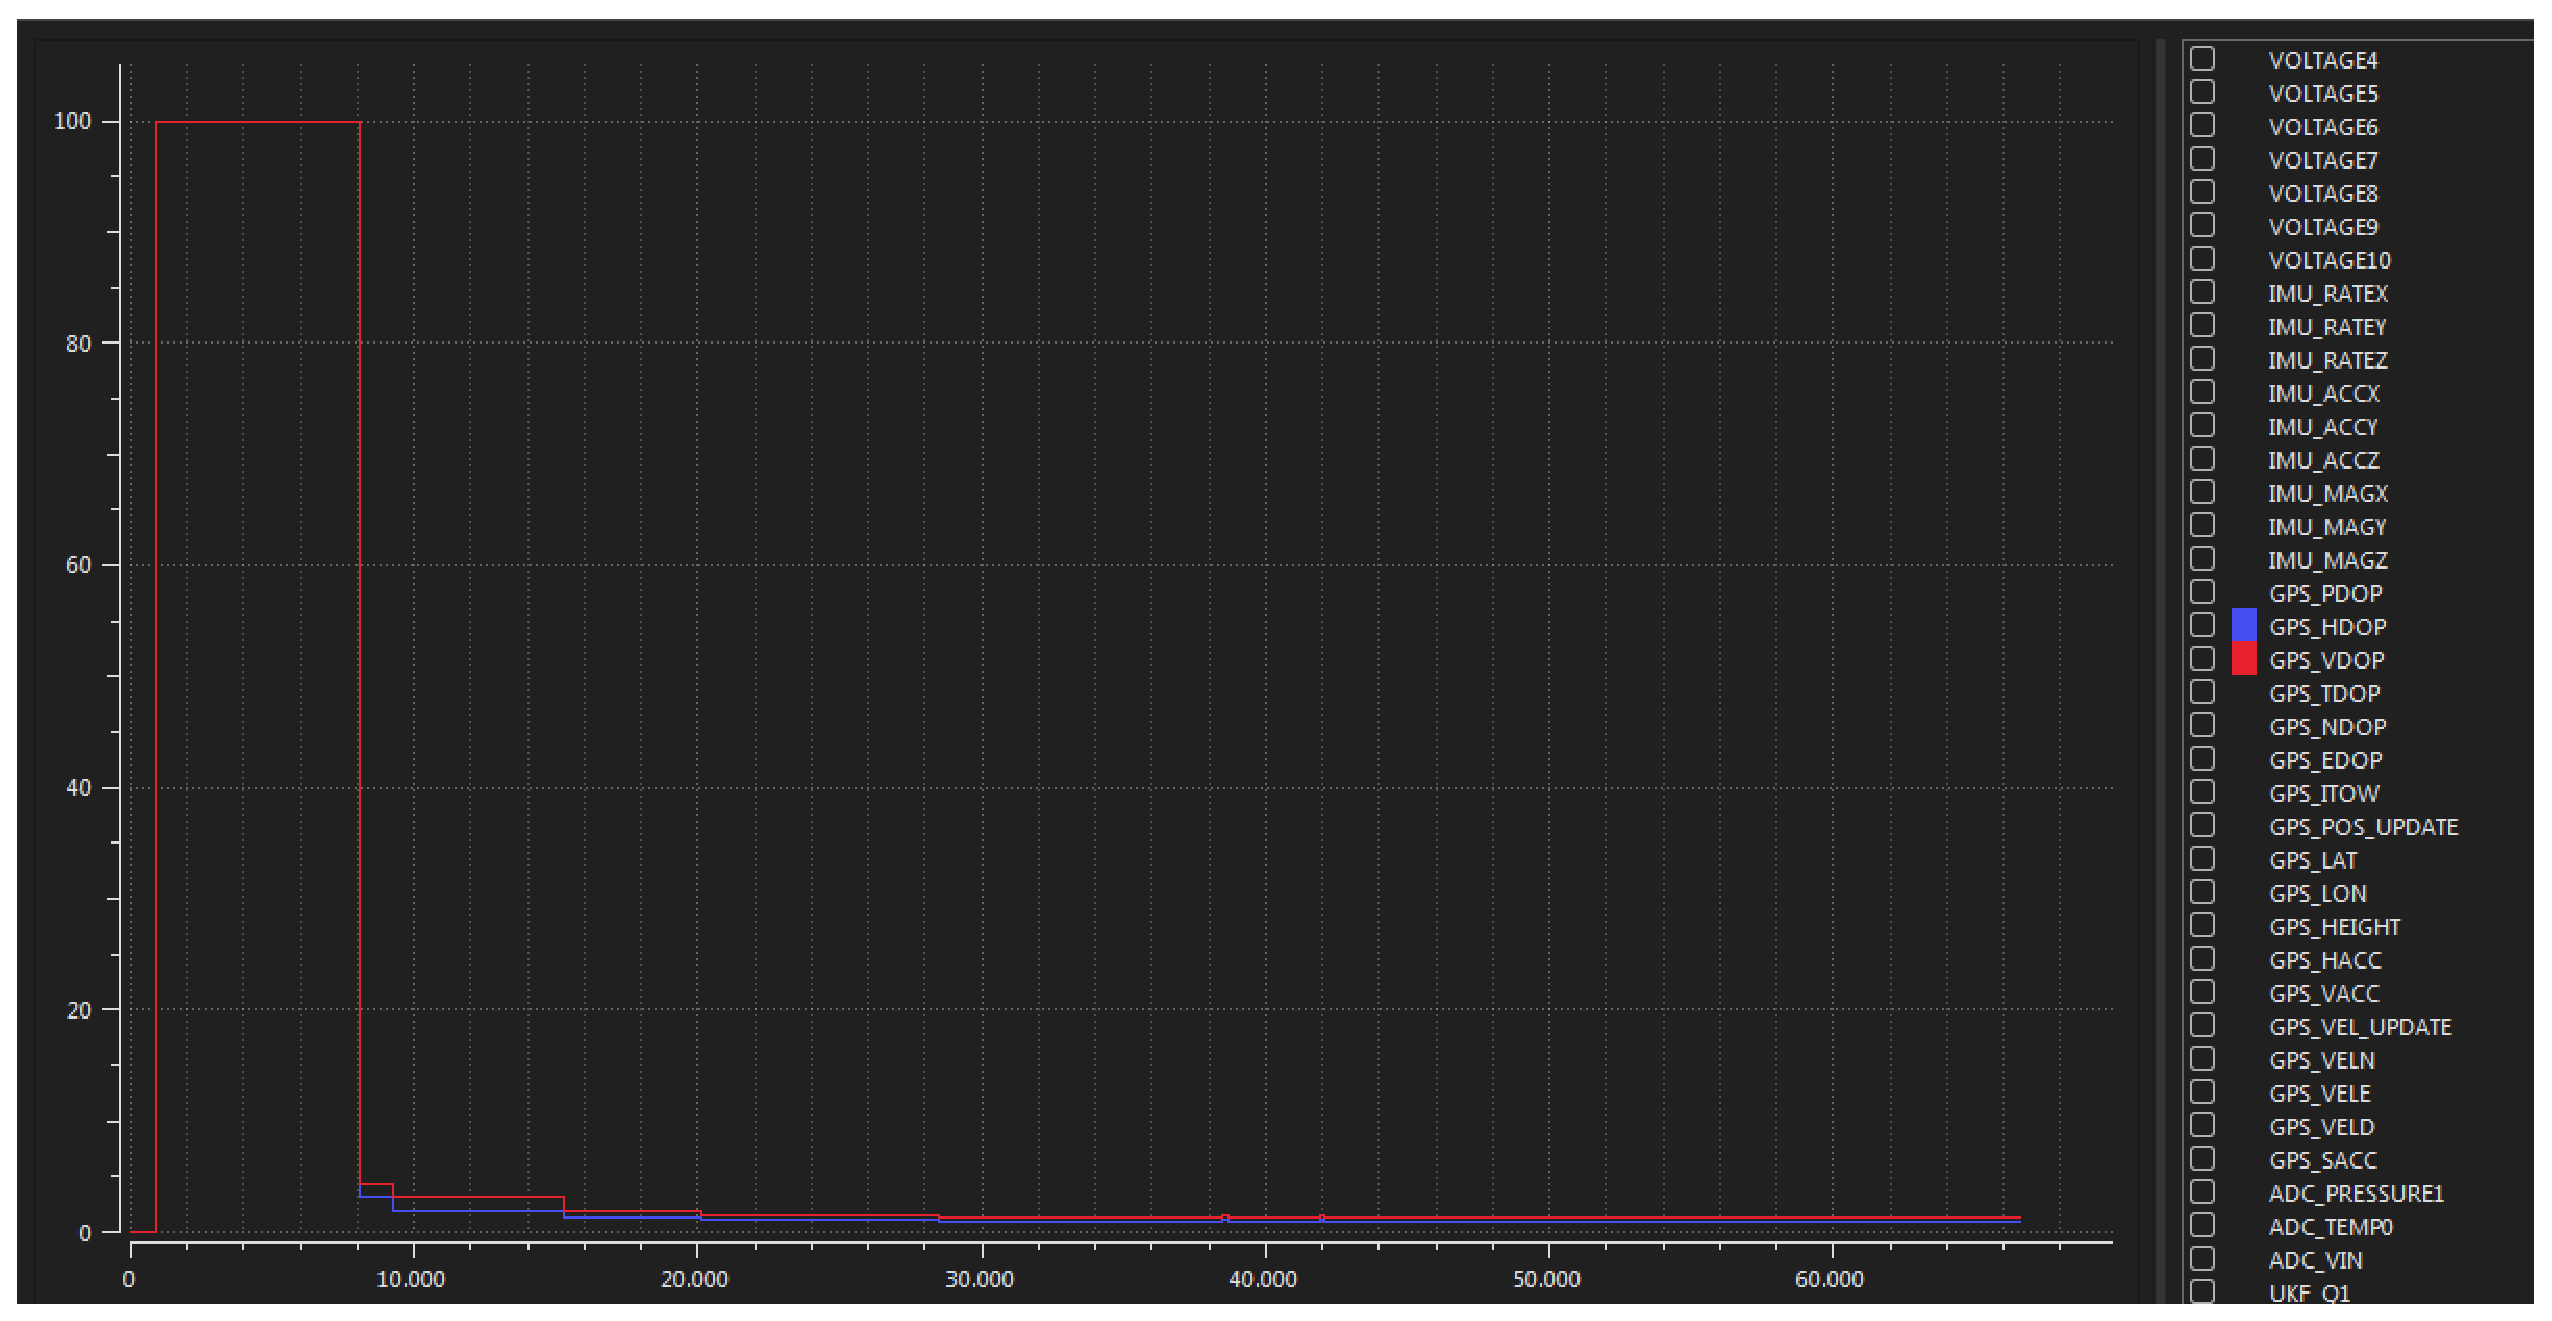
\includegraphics[width=1\textwidth]{graphics/test_qground_station_dop.eps}
  \caption{Plot of h/vDOP from logs when the drone was airborn}
    \label{fig:qground_station_dop}
\end{figure}

The test will be carried out again.
